% SPAR Final Report Draft
% To compile in an environment with TeX Live:
%   latexmk -pdf report.tex

\documentclass[final]{sparreport}

\title{Representation Without Control: Testing the Realization Effect in Language Models}

\author{
  \textbf{Ciar\'an Walsh and Emilio Barkett}
}

\sparround{Spring 2026}

\graphicspath{{figures/}{../../results/final/report_realization_v1/figures/}{results/final/report_realization_v1/figures/}}

\begin{document}

\maketitle

\begin{abstract}
Large language models are increasingly used as behavioral simulators, but it remains unclear when their choices reflect human-like cognitive mechanisms rather than prompt-sensitive surface patterns. We study the realization effect, a behavioral-economics finding in which risk-taking differs after paper versus realized gains and losses. We adapt casino and investment-style realization scenarios into prompts that elicit a wager and risk preference. Initial prompt-only results showed systematic condition sensitivity, but follow-up analyses did not support a clean replication of the human realization-effect pattern. We then analyzed Gemma residual-stream activations and found that a train-only realization direction separates realized/closed outcomes from paper/open outcomes on held-out prompts, including newly generated DeepSeek-authored prompts. However, activation steering along this train-only layer-18 realization direction did not reliably shift downstream risk choices, including in a negative sign-symmetry run. These results suggest a representation-behavior dissociation: models may encode semantically meaningful state variables without those variables being sufficient causal levers for the measured behavior.
\end{abstract}

\keywords{language models \and behavioral evaluation \and mechanistic interpretability \and activation steering \and risk-taking}

\section{Introduction}

Large language models (LLMs) are often used, implicitly or explicitly, as behavioral subjects. They answer survey questions, simulate agents, generate forecasts, and stand in for human respondents in early-stage social-science or policy experiments. This creates a methodological problem for AI safety and behavioral modeling: a model may produce responses that look psychologically meaningful without implementing anything like the human mechanism that originally motivated the task.

We study this problem through the realization effect. In human decision-making, risk-taking can depend on whether prior gains or losses are still paper outcomes in an open account or have been realized by closing the account. Imas~\cite{imas2016realization} showed that realized versus paper losses can induce different subsequent risk attitudes. Flepp, Meier, and Franck~\cite{flepp2021paper} studied related dynamics in casino gambling, and Merkle, M{\"u}ller-Dethard, and Weber~\cite{merkle2021closing} extended the question to gains as well as losses.

Our original question was behavioral: do LLMs reproduce the realization effect? As the project developed, the more informative question became mechanistic: if realization status matters in behavior, can we find a corresponding internal representation, and does intervening on that representation change risk choices?

We test three linked questions. First, do prompt-only LLM responses show sensitivity to paper/open versus realized/closed framing? Second, is realization status linearly readable from model activations, including on held-out prompts? Third, does steering along such a realization direction causally change wager or risk preference? The answer we find is mixed. Prompt-only behavior is condition-sensitive but does not robustly match the human realization-effect predictions. Gemma contains a readable realization direction in its residual stream, and a train-only direction generalizes to held-out readout prompts. Yet steering that train-only layer-18 realization direction does not reliably move downstream risk behavior. The final contribution is therefore not a successful behavioral replication, but a case study in representation without control.

\section{Related Work}

\subsection{The realization effect}

The realization effect distinguishes paper outcomes from realized outcomes. A paper loss or gain remains inside an open mental account; a realized loss or gain has been closed out. Imas~\cite{imas2016realization} uses this distinction to reconcile conflicting findings about whether prior losses increase or decrease risk-taking. Flepp et al.~\cite{flepp2021paper} provide field evidence from casino gambling, a setting in which within-visit paper outcomes and across-visit realized outcomes can be separated. Merkle et al.~\cite{merkle2021closing} study whether similar mental-account closure effects apply to both gains and losses.

This literature gives a useful benchmark for LLM behavioral evaluation because it makes directional predictions about a subtle latent variable: the same monetary outcome should have different implications depending on whether it is still open or has been realized.

\subsection{LLMs as behavioral subjects}

Prior work has proposed using LLMs as simulated human or economic subjects~\cite{aher2023simulate,horton2023simulated}. Such experiments are attractive because they are cheap, reproducible, and easy to scale across conditions. But the same properties make them fragile. A model response may reflect instruction-following priors, formatting artifacts, learned associations in text, or numeric anchors rather than a stable decision mechanism. For that reason, behavioral prompting alone is weak evidence that a model represents, uses, or reasons with the intended latent variable.

\subsection{Activation readout and steering}

Mechanistic interpretability offers a way to move beyond prompt-level behavior. Linear probes and contrastive activation directions can identify variables represented in a model's hidden states. Activation steering methods then test whether adding such a direction during inference changes behavior~\cite{turner2023activation,zou2023representation}. This is a stronger causal test than readout alone. At the same time, linear representation is not automatically behavioral control: a direction can encode information without being the relevant downstream policy variable~\cite{park2024linear}. Our experiment is designed around this gap.

\section{Methods}

\subsection{Prompt-only behavioral task}

We constructed vignette prompts modeled on the realization-effect literature. The original prompt-only dataset uses 11 conditions spanning paper outcomes and realized outcomes, with both absolute-outcome and balance-relative prompt versions. The model is asked to return two integers: a next-session wager from 1 to 1000 CHF and a slot-machine risk preference from 1 to 5. The cleaned dataset contains 46,750 rows, of which 45,865 have valid parsed wagers and 45,808 have valid risk-profile responses.

We analyze two outcomes: log wager and risk profile. The main regressions use condition indicators with model, temperature, and prompt-version fixed effects, and HC3 robust standard errors. Paper conditions are compared against a paper-even baseline, while realized conditions are compared against a small realized-loss baseline.

\subsection{Activation-vector prompt set}

For the mechanistic pass, we generated paired prompts contrasting \texttt{paper\_open} and \texttt{realized\_closed} framings across several realization-status domains, including finance, reimbursement, budget, compensation, academic, project-outcome, and casino scenarios. The behavior-evaluation subset is narrower: it contains casino and finance prompts that ask for downstream wager or investment-risk choices. We logged Gemma residual-stream activations and constructed a mean-difference direction:
\[
v_{\mathrm{realization}} = \mu_{\mathrm{realized\_closed}} - \mu_{\mathrm{paper\_open}}.
\]
The main readout and risk-behavior steering artifact is the layer-18 direction from local Gemma 3 4B computed using only the \texttt{direction\_train} split: 756 matched paper/realized pairs. We evaluated that frozen train-only direction on the original \texttt{direction\_val} and \texttt{behavior\_eval} splits, plus a newly generated DeepSeek-authored held-out prompt set. The DeepSeek set contains 40 matched pairs split into \texttt{heldout\_readout} and \texttt{heldout\_behavior\_eval}; neutral outcome cells were omitted because preliminary generation made neutral wording ambiguous. Some earlier descriptive activation plots use the all-pairs layer-18 direction from the original activation run and are labeled as descriptive rather than strict held-out evidence.

\subsection{Steering intervention}

We implemented a local residual-stream steering runner for Gemma. During generation, a forward hook adds a scaled, normalized realization direction at a selected layer. The full risk-behavior run reported here steers the train-only layer-18 direction at the final active token position using scales \(-50\), \(0\), \(+50\), \(+75\), \(+100\), and \(+150\). Positive scales point toward \texttt{realized\_closed}; negative scales point toward \texttt{paper\_open}. The run uses the same 648 behavior-evaluation prompts at each scale and compares steered responses to the in-run unsteered scale-\(0\) baseline on matched prompt IDs.

We report both all matched valid rows and an exactly-two-integer subset where the response contains exactly two integer tokens. This subset is important because steering sometimes perturbs the answer contract, and parsing failures can create misleading numeric outcomes.

\subsection{Positive-control classification steering protocol}

To test whether a realization direction can move a direct semantic judgment even when wager control is weak, we created a paired classification task from the same behavior-evaluation prompts. Instead of returning wager and risk integers, the model is asked to classify each scenario as \texttt{REALIZED} or \texttt{PAPER}. This diagnostic classification run used the earlier all-pairs layer-18 direction and evaluated three steering scales (\(-100\), \(0\), \(+100\)) on all 648 behavior-evaluation prompts.

Because free generation often adds extra text, we score label candidates directly from token log-probabilities under steering hooks and choose the higher-scoring label. Scores are length-normalized and prior-calibrated within scale, then summarized by accuracy and realized-prediction rate. The current scored run has one prompt-construction caveat: the classification instruction was present in the prebuilt classification prompt CSV and was then added again by the steering runner, so these positive-control results should be treated as diagnostic rather than final.

\section{Results}

\subsection{Prompt-only behavior is condition-sensitive but not a clean realization-effect replication}

The prompt-only behavioral data show systematic responses to outcome framing, but not in the clean pattern predicted by the human realization-effect literature. In the cleaned regular prompting dataset, paper-outcome effects on \texttt{risk\_profile} are mostly positive relative to the paper baseline: paper large losses, paper medium losses, paper small gains, and paper large gains all increase the risk-profile measure, while paper small losses do not significantly differ from baseline. However, wager effects are mixed. For \texttt{log\_wager}, paper large losses increase wagers, while paper medium losses, paper small losses, and paper gains decrease wagers.

The realized-outcome results diverge more sharply from the original human prediction. Realized losses increase rather than decrease both log wager and risk profile relative to the small realized-loss baseline. Realized gains also differ significantly from baseline. These patterns suggest that LLMs are sensitive to outcome magnitude and framing, but the response is not well described as a faithful realization-effect replication.

\begin{figure}[htbp]
  \centering
  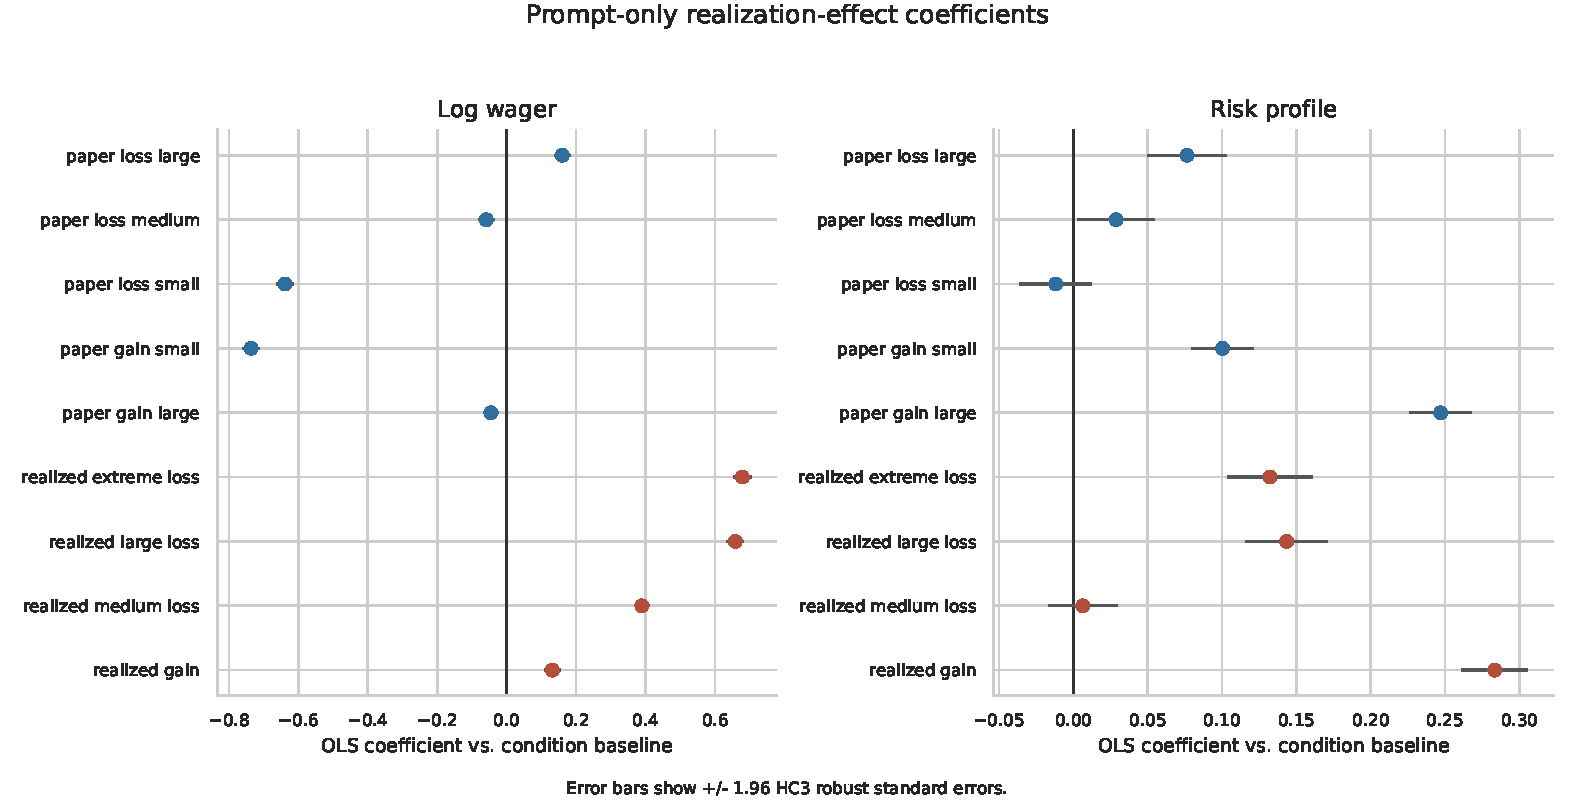
\includegraphics[width=\textwidth]{behavioral_coefficients.pdf}
  \caption{Prompt-only behavioral coefficients from the cleaned realization-effect dataset. Points show OLS condition coefficients; error bars show approximate 95\% intervals using HC3 robust standard errors. The model is condition-sensitive, but the coefficient pattern does not cleanly match the original human realization-effect predictions.}
  \label{fig:behavioral-coefficients}
\end{figure}

\subsection{Gemma has a readable realization representation}

The activation analysis gives the positive mechanistic result. Along the layer-18 mean-difference direction, \texttt{paper\_open} and \texttt{realized\_closed} prompts separate across the logged activation set, including the behavior-evaluation prompts used later for steering. The original visualization in Figure~\ref{fig:activation-projection} uses the all-pairs readout artifact, so it should be read as a descriptive projection plot rather than the strict generalization test.

The stricter check is the train-only readout analysis. A direction built only from the 756 \texttt{direction\_train} pairs still separates realized/closed from paper/open prompts on the original held-out validation split and on the newly generated DeepSeek held-out set. The result is strongest for the direction-style prompts and weaker for behavior-evaluation prompts, especially in the small DeepSeek behavior subset, but all evaluated splits have positive realized-minus-paper mean projection deltas.

\begin{figure}[htbp]
  \centering
  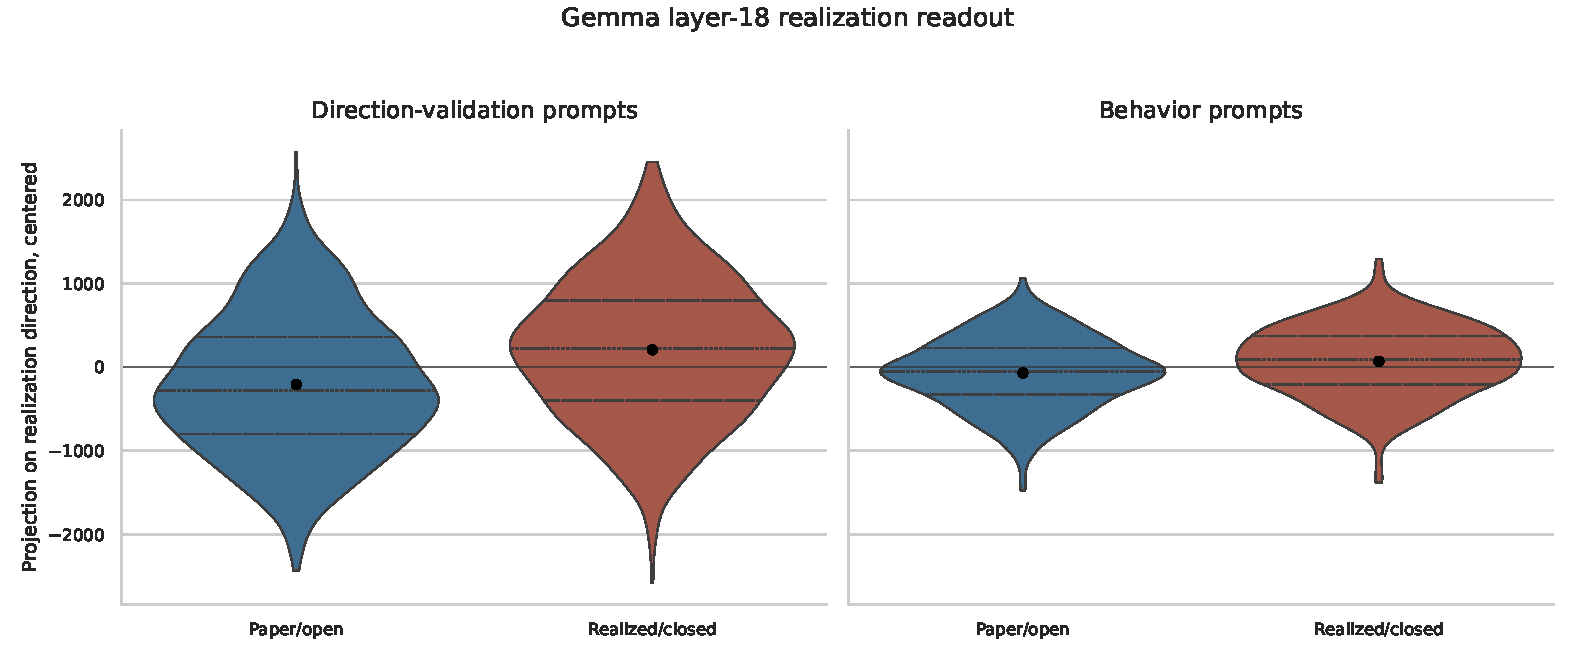
\includegraphics[width=\textwidth]{activation_projection_layer18.pdf}
  \caption{Gemma layer-18 projections on the realization direction. Projections are centered within split for readability. Realized/closed prompts shift upward relative to paper/open prompts, supporting the claim that realization status is linearly readable in the logged residual-stream activations.}
  \label{fig:activation-projection}
\end{figure}

\begin{table}[htbp]
  \centering
  \small
  \caption{Train-only layer-18 readout evaluated on original and DeepSeek-authored prompt splits. Correct direction is the percentage of matched pairs where the realized/closed prompt projects higher than the paper/open prompt.}
  \label{tab:heldout-readout}
  \begin{tabular}{llrrr}
    \toprule
    Dataset & Split & Pairs & Mean projection delta & Correct direction \\
    \midrule
    Original & \texttt{direction\_train} & 756 & 417.36 & 89.2\% \\
    Original & \texttt{direction\_val} & 756 & 413.43 & 91.1\% \\
    Original & \texttt{behavior\_eval} & 324 & 137.19 & 80.6\% \\
    DeepSeek held-out & \texttt{heldout\_readout} & 28 & 443.62 & 92.9\% \\
    DeepSeek held-out & \texttt{heldout\_behavior\_eval} & 12 & 123.08 & 75.0\% \\
    \bottomrule
  \end{tabular}
\end{table}

\subsection{Projection strength is weakly linked to behavior}

We next asked whether stronger projection on the realization direction predicts the model's actual wager or risk response. At the raw prompt level, projection is positively associated with wager: a one-standard-deviation increase in projection predicts an 84.44 CHF larger wager (\(p < 10^{-5}\)). Projection also weakly predicts risk profile (\(+0.136\) on the 1--5 scale, \(p = 0.021\)). However, this relationship mostly reflects prompt structure. After controlling for pair role, domain, outcome valence, amount bucket, and prompt source, the projection coefficient for wager falls to \(+5.21\) CHF and is not significant (\(p = 0.776\)). The risk-profile coefficient remains marginal (\(+0.134\), \(p = 0.053\)), but the model explains little variance.

The stricter within-pair analysis is more important for the representation-without-control claim. For each matched pair, we computed the realized-minus-paper projection delta and compared it with the realized-minus-paper wager and risk deltas. Projection deltas barely predict behavior deltas: Pearson \(r = 0.072\) for wager and \(r = 0.001\) for risk. Regressions with prompt controls likewise do not find reliable effects. Thus, the activation direction tracks realization status, but variation in projection strength does not robustly explain variation in downstream risk behavior.

\begin{figure}[htbp]
  \centering
  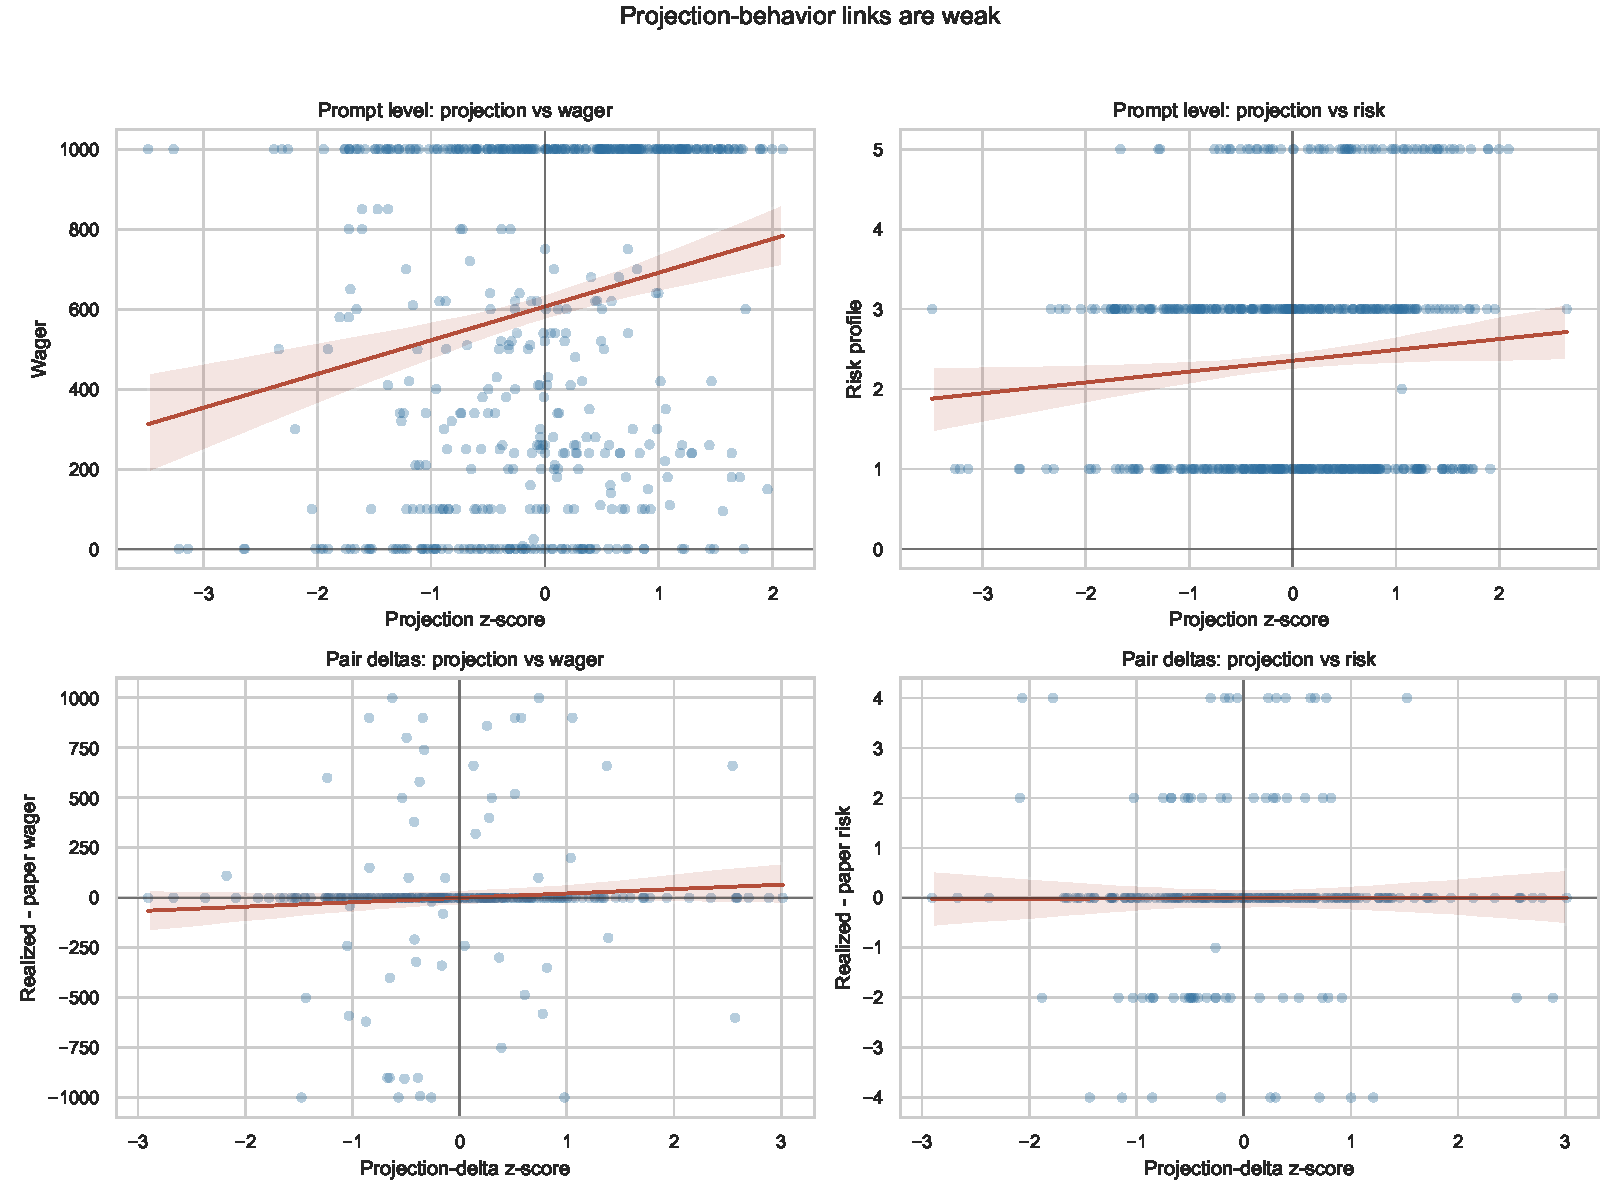
\includegraphics[width=\textwidth]{projection_behavior_link.pdf}
  \caption{Projection strength versus behavior. Raw prompt-level projection has a positive association with wager, but within matched paper/realized pairs, projection deltas weakly predict wager deltas and essentially do not predict risk deltas. This supports the distinction between readable representation and behavioral control.}
  \label{fig:projection-behavior}
\end{figure}

\subsection{Steering does not robustly control risk behavior}

If the layer-18 realization direction were a simple causal lever for risk-taking, steering toward \texttt{realized\_closed} should move behavior in one direction and steering toward \texttt{paper\_open} should move it in the opposite direction. We do not observe this pattern.

Across positive scales \(+50\), \(+75\), \(+100\), and \(+150\), mean wager deltas are small and positive, but median deltas are zero. Mean risk-profile deltas remain close to zero, with small negative movement at larger positive scales. The negative sign-symmetry run at \(-50\) also fails to produce a clean opposite-direction behavioral effect: it has an exactly-two-integer matched mean wager delta of \(+7.22\), an exactly-two-integer matched mean risk delta of \(+0.057\), and median deltas of zero for both outcomes. This makes it difficult to interpret the steering response as directional control over risk behavior.

\begin{table}[htbp]
  \centering
  \caption{Matched steering deltas relative to the in-run unsteered Gemma behavior baseline. The table reports all valid matched rows from the train-only layer-18 steering run. Exactly-two-integer rows show the same qualitative result: small mean shifts and zero median shifts.}
  \label{tab:steering-deltas}
  \begin{tabular}{rrrrr}
    \toprule
    Scale & Matched rows & Mean wager delta & Mean risk delta & Median deltas \\
    \midrule
    -50 & 478 & 11.80 & 0.094 & 0 / 0 \\
     50 & 476 & 7.24 & 0.013 & 0 / 0 \\
     75 & 483 & 8.21 & -0.025 & 0 / 0 \\
    100 & 478 & 15.24 & -0.050 & 0 / 0 \\
    150 & 473 & 12.80 & -0.080 & 0 / 0 \\
    \bottomrule
  \end{tabular}
\end{table}

\begin{figure}[htbp]
  \centering
  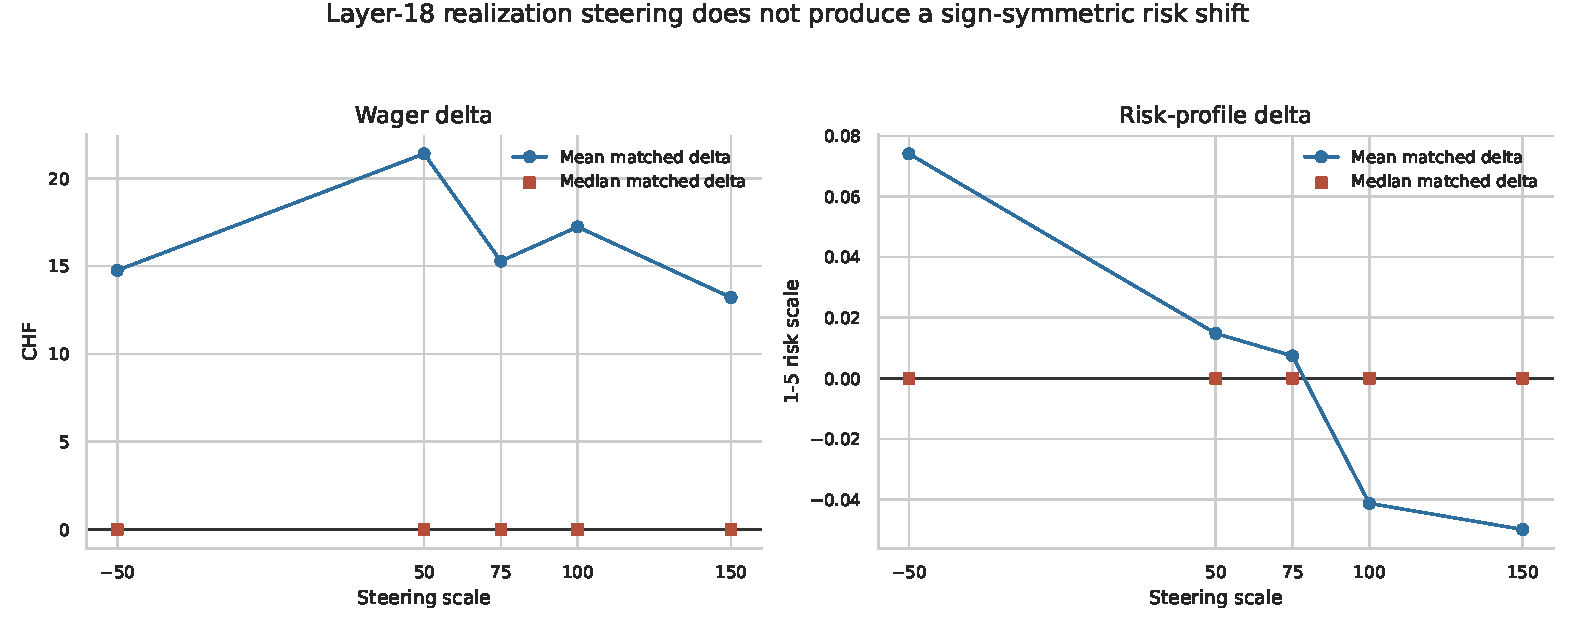
\includegraphics[width=\textwidth]{steering_dose_response.pdf}
  \caption{Dose-response plot for Gemma train-only layer-18 realization steering on the exactly-two-integer matched subset. The negative scale does not produce a clean behavioral reversal, and median matched deltas remain zero across wager and risk outcomes.}
  \label{fig:steering-dose}
\end{figure}

\subsection{Positive-control classification steering shows only weak directional movement}

We ran a full positive-control pass on the direct \texttt{REALIZED}/\texttt{PAPER} classification task (648 prompts per scale; 1,944 rows total). The steering direction does induce a small directional movement: the realized-prediction rate increases from \(0.140\) at unsteered scale \(0\) to \(0.198\) at \(+100\), and decreases to \(0.120\) at \(-100\). However, classification accuracy remains near chance overall (\(0.520\) at scale \(0\), \(0.515\) at \(+100\), \(0.512\) at \(-100\)).

The prediction breakdown clarifies why this is weak evidence of usable control. The label set is balanced, but the model strongly favors \texttt{PAPER}. Across all scales, \texttt{paper\_open} prompts are usually classified correctly (accuracy \(0.863\)), while \texttt{realized\_closed} prompts are rarely classified correctly (accuracy \(0.169\)). Thus, even in a direct semantic task, steering produces only modest directional shifts and does not yield robust controllability.

\subsection{Compliance artifacts matter}

Steering also affects answer-contract compliance. The task asks for exactly two integers, and many responses either contain too few or too many integer tokens for unambiguous parsing. This matters because parsed numeric outcomes are only meaningful when the answer contract is followed. Noncompliance is concentrated in prompts generated from the Sonnet source, which fail the exactly-two-integer criterion at much higher rates than the GPT-5.4 prompt source and usually higher rates than the Grok-fast prompt source. At \(-50\), for example, Sonnet-derived prompts have 106 noncompliant responses out of 216, compared with 46/216 for GPT-5.4-derived prompts and 70/216 for Grok-fast-derived prompts.

\begin{figure}[htbp]
  \centering
  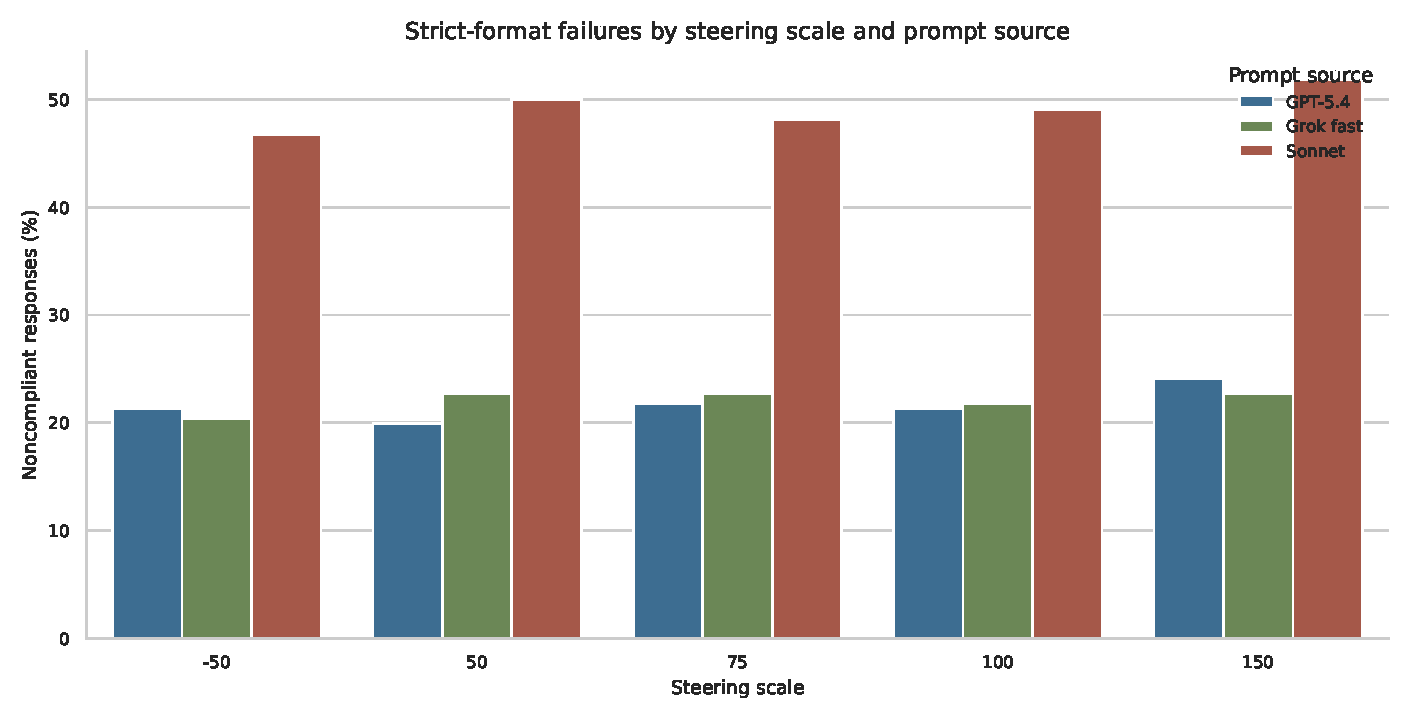
\includegraphics[width=0.92\textwidth]{compliance_by_scale.pdf}
  \caption{Exactly-two-integer noncompliance by steering scale and prompt source. The Sonnet-derived prompt subset has substantially higher failure rates, motivating exactly-two-integer subset analyses and caution in interpreting small mean shifts.}
  \label{fig:compliance}
\end{figure}

\begin{table}[htbp]
  \centering
  \small
  \caption{Hypothesis outcome summary.}
  \label{tab:hypothesis-summary}
  \begin{tabular}{p{0.26\textwidth}p{0.15\textwidth}p{0.49\textwidth}}
    \toprule
    Test & Outcome status & Evidence summary \\
    \midrule
    Prompt-only behavioral replication & Partial / weak & Condition sensitivity is clear, but directional patterns do not robustly match human realization-effect predictions. \\
    Activation readout (layer-18 direction) & Supported / held-out readout & A train-only direction separates realized/closed from paper/open prompts on original validation prompts and on a newly generated DeepSeek held-out readout set. \\
    Projection strength versus behavior & Weak / mixed & Raw prompt-level association exists, but within-pair projection deltas weakly predict wager/risk deltas. \\
    Risk-behavior steering intervention & Not supported & Steering shifts are small, medians are zero, and negative-scale symmetry does not produce a clean reversal. \\
    Positive-control classification steering & Weak diagnostic support & Directional shift in realized-prediction rate occurs (\(-100 < 0 < +100\)), but accuracy remains near chance with a strong \texttt{PAPER} prediction bias and a duplicated-instruction caveat. \\
    \bottomrule
  \end{tabular}
\end{table}

\section{Discussion}

The strongest conclusion is a representation-behavior dissociation. Gemma appears to encode whether an outcome is realized/closed or paper/open, and this readout generalizes beyond the prompts used to build the train-only direction. However, the corresponding activation direction does not reliably control downstream risk choices in our assay. This distinction matters for both behavioral evaluation and mechanistic interpretability.

For behavioral evaluation, the prompt-only results warn against interpreting LLM condition sensitivity as human-like cognition. The models react to prior outcomes, but the direction and outcome dependence do not reproduce the intended mental-accounting pattern. For mechanistic interpretability, the steering results warn against treating linear decodability as explanation. A feature can be readable in residual activations while still failing to act as a simple causal control variable for the behavior of interest.

There are several possible interpretations. The realization direction may encode semantic status without connecting to the model's numeric decision policy. Risk choices may be dominated by other factors such as instruction following, learned defaults for conservative or aggressive gambling advice, prompt-source artifacts, or numeric anchors. The layer-18 intervention may also be too narrow: a different layer, position mode, or multi-layer intervention could have stronger effects. However, the sign-symmetry result makes the simplest causal story less plausible. Pushing in the negative direction did not produce an opposite behavioral shift.

\section{Limitations}

This report should not be read as proving that realization status never causally affects LLM risk behavior. The intervention is limited to local Gemma 3 4B, layer 18, a normalized train-only mean-difference direction, and final-token steering. We have not completed a full layer sweep, a position-mode sweep, or multi-layer steering. Hosted Qwen behavior runs can test prompt-only replication, but they cannot support residual-stream steering through API access because hidden states and generation hooks are not exposed.

The behavioral assay is also indirect. Wager and risk-profile answers are constrained numeric outputs, which makes the task easy to score but may amplify format and parsing artifacts. Exactly-two-integer compliance is imperfect, especially for Sonnet-derived prompts. The regular prompt-only dataset pools 25 models, so the aggregate coefficients should be read alongside per-model robustness rather than as evidence that every model behaves the same way. Finally, the held-out readout reduces leakage concerns for the representation claim, but the direction may still encode a broad semantic contrast rather than the exact decision-relevant variable that would change risk-taking.

The new DeepSeek held-out set is also small and single-source. It is useful because it was not used to build the direction and passed a local overlap audit against the original prompt set, but it should not be treated as exhaustive evidence across prompt generators, domains, or behavior tasks. The \texttt{heldout\_behavior\_eval} split currently tests projection separation, not newly generated downstream Gemma wager or risk responses.

The steering summaries report matched mean and median deltas, but they do not yet include bootstrap or randomization intervals for those deltas. The zero medians, small mean effects, and lack of a clean sign-symmetric behavioral response are the main evidence against robust control, but interval estimates would make the null result easier to calibrate.

\section{Future Work}

The next intervention step is to improve causal leverage, not just detect directional movement. The train-only held-out readout and train-only layer-18 risk-behavior steering run are now in place, and the result still does not support robust behavioral control. The diagnostic positive-control classification pass suggests the current single-layer, single-position intervention is too weak for robust semantic control, though it should be rerun with the train-only direction and corrected prompt construction. Immediate follow-up should test layer sweeps around 14, 16, 18, 20, and 22, plus \texttt{position\_mode=all} and multi-layer steering schedules.

A second priority is to expand held-out evaluation. The current DeepSeek set is enough to support a cautious held-out readout claim, but future work should add more source models, larger behavior-evaluation subsets, and newly generated Gemma responses for those held-out behavior prompts. A third priority is cross-model intervention replication under the same local-hook framework. Building a local Qwen activation pipeline would allow direct comparison of readout and steering behavior across architectures without API-level hidden-state constraints. Finally, the report package should add appendix robustness tables for prompt-source stratification, overlap-audit results, and exactly-two-integer sensitivity.

\section{Conclusion}

We began by asking whether LLMs reproduce the realization effect in risk-taking. The answer from the current evidence is no, at least not robustly. Prompt-only behavior is condition-sensitive, but it does not cleanly match the human realization-effect predictions. Gemma contains a readable realization representation in its layer-18 residual stream, and this representation is visible on held-out readout prompts. But steering along a realization direction does not reliably change wager or risk choices. This makes the project useful as a negative result: it clarifies the gap between observing behavior, decoding an internal representation, and demonstrating causal control. In this case, realization status is represented, but representation is not enough.

\bibliographystyle{plain}
\bibliography{references}

\end{document}
